% Revised Results - Publication Quality
% Clear narrative structure with meaningful section names

\section{Results}
\label{sec:results}

We first report the primary cross-view result under task-sufficient observation. We then locate its boundary under critical sensor loss, interpret that boundary with an exploratory oracle comparison, and separate geometric behavior from predictive quality and calibration. The section closes with a complementary shared-model evaluation on C-MAPSS. Unless stated otherwise, intervals in the synthetic analyses use 2,000 asset-level bootstrap replicates.

\subsection{Cross-View Consistency Under Sufficient Observation}
\label{sec:results:sufficient}

\subsubsection{Primary Finding}

When observation processes maintain task sufficiency---that is, when different sensor subsets all support reliable RUL prediction---PROP-DIRECT substantially reduces posterior inconsistency across views of the same asset. Table~\ref{tab:c1_resolution} reports the formal lockbox validation results.

\begin{table}[tb]
  \centering
  \caption{Resolution sensitivity on the lockbox split. Intervals are
  two-sided 90\% bootstrap confidence intervals with 2,000 replicates.}
  \label{tab:c1_resolution}
  \begin{tabular}{lccc}
    \toprule
    Sampling budget & PROP-DIRECT geometry & Relative reduction & 90\% CI \\
    \midrule
    256 (primary) & 0.0002864 & 38.64\% & [34.78\%, 42.44\%] \\
    64 (check)    & 0.0002849 & 38.97\% & [35.03\%, 42.66\%] \\
    \bottomrule
  \end{tabular}
\end{table}

% Table: Baseline Consistency Comparison
% Addresses P0-2: Shows improvement is robust across baseline choices

\begin{table}[t]
\centering
\begin{threeparttable}
\caption{\textbf{Geometric consistency comparison across baselines.}
Energy distance for PROP-DIRECT and two observation-agnostic baselines
under the sufficient observation regime. Relative reduction computed as
$(d_E(\text{baseline}) - d_E(\text{PROP})) / d_E(\text{baseline}) \times 100\%$.
Lower energy distance indicates better cross-view posterior consistency.
Both baselines yield comparable absolute energy distance, confirming
that relative improvements are robust to baseline choice.}
\label{tab:baseline_comparison}
\begin{tabular}{llcc}
\toprule
\textbf{Split} & \textbf{Model} & \textbf{Energy Distance} & \textbf{Relative Reduction} \\
\midrule
Test   & PROP-DIRECT  & $2.89 \times 10^{-4}$ & --- \\
       & B-STDPROB    & $4.57 \times 10^{-4}$ & 36.8\% \\
       & B-INDEP      & $4.66 \times 10^{-4}$ & 38.0\% \\
\midrule
Lockbox & PROP-DIRECT  & $2.86 \times 10^{-4}$ & --- \\
        & B-STDPROB    & $4.64 \times 10^{-4}$ & 38.3\% \\
        & B-INDEP      & $4.67 \times 10^{-4}$ & 38.6\% \\
\bottomrule
\end{tabular}
\begin{tablenotes}
\footnotesize
\item Bootstrap 90\% confidence intervals for the primary comparison
(PROP-DIRECT vs B-INDEP): Test [35.1\%, 40.7\%], Lockbox [34.8\%, 42.4\%].
B-STDPROB and B-INDEP differ by less than 1\% in absolute energy distance,
indicating that the choice of observation-agnostic baseline does not
materially affect conclusions.
\end{tablenotes}
\end{threeparttable}
\end{table}


The architecture achieves an absolute geometry metric of $2.86 \times 10^{-4}$ on the lockbox split, well below the pre-specified acceptability threshold of $3.5 \times 10^{-4}$. More importantly, this represents a \textbf{38.6\% reduction} (90\% CI: 34.8--42.4\%) in cross-view inconsistency relative to the observation-agnostic baseline (B-INDEP). The test split yields a consistent 38.1\% reduction (90\% CI: 34.2--41.9\%), confirming the effect is not an artifact of a single data partition.

Because a small cross-view distance can also result from an invariant predictor, we
additionally inspected the frozen oracle-relative quantity defined in
Section~\ref{sec:methods:metrics}. On the lockbox split, the asset-level mean
$E_{\mathrm{geometry}}$ was $8.07\times10^{-4}$ for PROP-DIRECT and
$9.29\times10^{-4}$ for B-STDPROB; the corresponding test values were
$6.89\times10^{-4}$ and $7.96\times10^{-4}$. These are descriptive post-hoc
summaries, not a replacement for the preregistered consistency endpoint; the
asset-bootstrap comparison for the information-loss regimes is reported later in
Table~\ref{tab:oracle_alignment}.

Figure~\ref{fig:c1-forest} visualizes the same effect sizes and confidence
intervals. The close alignment of the test and lockbox estimates makes the
replication pattern visible without relying on a numerical comparison alone.

\begin{figure}[!ht]
  \centering
  \includegraphics[width=0.86\linewidth]{fig2_c1_main_result_forest.png}
  \caption{\textbf{Primary consistency result.} PROP-DIRECT reduces cross-view posterior
  inconsistency relative to B-INDEP by approximately 38\% on both the test and
  lockbox splits. Squares show point estimates and horizontal bars show 90\%
  bootstrap confidence intervals; the reduced 64-sample budget produces the same
  conclusion.}
  \label{fig:c1-forest}
\end{figure}

Predictions from different views of the same asset are therefore substantially closer in posterior geometry. The result motivates testing whether such alignment improves uncertainty-aware maintenance decisions, where prediction intervals and tail probabilities influence action.

\subsubsection{Robustness to Sampling Budget}

A critical deployment consideration is computational cost. Uncertainty quantification via Monte Carlo sampling typically dominates inference time, making sampling budget a key engineering constraint. We therefore evaluated whether the geometric improvement persists under reduced sampling.

When the Monte Carlo budget is reduced four-fold from 256 to 64 samples per prediction, the effect size changes by only 0.34 percentage points: 38.97\% reduction (90\% CI: 35.03--42.67\%) versus 38.64\% at the standard budget. This stability indicates that the geometric benefit does not rely on high-precision uncertainty estimation within the synthetic evaluation; whether this translates into an acceptable deployment latency trade-off requires a direct systems benchmark.

\subsubsection{Interpretation}

These results support the hypothesis that explicit observation-process conditioning enables models to align posterior geometry across compatible views. The architecture appears to learn that different sensor configurations, when task-sufficient, should produce posteriors that overlap appropriately rather than diverging arbitrarily. The robustness to sampling budget suggests this is a structural property of the learned representations, not a fragile artifact of estimation precision.

\subsection{Boundary Behavior Under Critical Sensor Loss}
\label{sec:results:boundary}

The boundary comparison defined in Section~\ref{sec:methods:protocol} holds the
number of deleted sensors fixed while changing their functional role. It asks
whether the conditioning pathway distinguishes a critical deletion from a matched
random deletion, rather than merely responding to the amount of missing data.

\subsubsection{The Importance Boundary}

PROP-DIRECT does \emph{not} outperform the baseline in this regime. Across three pre-registered estimands measuring different aspects of geometric inconsistency under information loss, all comparisons favor the baseline or show no advantage:

\begin{itemize}
    \item \textbf{Critical-sensor excess risk:} $\Delta R_{\text{crit}} = +8.65 \times 10^{-4}$ (90\% CI: 7.36--9.91 $\times 10^{-4}$)
    \item \textbf{Loss-geometry differential:} $\Delta G_{\text{loss}} = +1.88 \times 10^{-4}$ (90\% CI: $-3.55$ to $+6.99 \times 10^{-4}$)
    \item \textbf{Interaction effect:} $I_R = +7.68 \times 10^{-4}$ (90\% CI: 5.16--10.28 $\times 10^{-4}$)
\end{itemize}

All point estimates are positive, indicating PROP-DIRECT exhibits \emph{greater} inconsistency than the baseline under importance-dependent information loss. The confidence intervals either exclude zero or barely overlap it, providing consistent evidence against the superiority hypothesis.

\subsubsection{Predictive-quality guardrail}

The geometric degradation is accompanied by only a small change in predictive quality. A pre-specified guardrail based on continuous ranked probability score (CRPS)---a proper scoring rule for probabilistic forecasts---gives: $\Delta \text{CRPS} = +4.07 \times 10^{-4}$ (90\% CI: $-0.22$ to $+8.47 \times 10^{-4}$), well below the non-inferiority margin of $3.85 \times 10^{-3}$.

The two metrics therefore capture different aspects of the model: the limitation concerns \emph{geometric consistency}, while single-view RUL prediction remains competitive.

\subsubsection{Pair-Class Decomposition}

Examining the three comparison types reveals structure in the failure:

Figure~\ref{fig:c2-pairs} provides a visual summary of the pair-class ordering
before the numerical decomposition below.

\begin{figure}[!ht]
  \centering
  \includegraphics[width=0.75\linewidth]{fig3_c2_pair_class_decomposition.png}
  \caption{\textbf{Information-loss pair-class decomposition.} Excess inconsistency relative
  to B-STDPROB is small for critical-versus-full comparisons but substantially
  larger for the matched-random class. The associated win rates show the same
  ordering, highlighting the pair class in which the current flat sensor-set
  representation is least effective.}
  \label{fig:c2-pairs}
\end{figure}

\begin{center}
\begin{tabular}{lcc}
\toprule
Comparison & Mean Difference & PROP-DIRECT Win Rate \\
\midrule
Critical vs. Full (parent) & $+2.8 \times 10^{-5}$ & 48\% \\
Critical vs. Random (matched) & $+3.72 \times 10^{-4}$ & 39\% \\
Critical vs. Redundant & $+1.64 \times 10^{-4}$ & 42\% \\
\bottomrule
\end{tabular}
\end{center}

The pair-class ordering is informative: PROP-DIRECT is nearly at parity with the
baseline for critical deletion versus the full sensor complement ($+2.8 \times
10^{-5}$ mean difference; 48\% win rate), whereas its excess inconsistency is
larger for random and redundant deletions. The matched-random comparison carries
the largest excess inconsistency and the lowest win rate, making it the clearest
stress test of whether sensor identity, rather than sensor count alone, is
represented.

Figure~\ref{fig:c2-pairs} makes this asymmetry explicit: the matched-random
comparison has the largest excess inconsistency and the lowest PROP-DIRECT win
rate, supporting the interpretation that the architecture detects missing
information more readily than functional sensor importance.

Figure~\ref{fig:prediction-example} makes this contrast concrete for one asset at
one query time: removing ancillary sensors leaves the posterior nearly unchanged,
whereas removing a critical sensor widens and shifts the distribution.

\begin{figure}[!ht]
  \centering
  \includegraphics[width=0.86\linewidth]{fig6_prediction_example.png}
  \caption{\textbf{Illustrative prediction under changing sensor sets.} For the
  same asset and query time, full sensors and ancillary-sensor removal produce
  closely overlapping posteriors, while critical-sensor removal yields a wider
  and shifted distribution. The example gives an operational interpretation of
  cross-view consistency and its importance-dependent boundary.}
  \label{fig:prediction-example}
\end{figure}

\FloatBarrier

\subsection{Exploratory Mechanistic Analysis}
\label{sec:results:mechanism}

\subsubsection{Motivation and Scope}

The boundary-regime results suggest PROP-DIRECT can detect that information has changed (near-parity vs. full sensor complement) but struggles when functional importance matters (poor performance vs. matched random deletion). To investigate this mechanism, we conducted a post-hoc exploratory analysis examining how model predictions track oracle-defined task difficulty. This analysis was \emph{not} part of the pre-registered decision criteria and should be interpreted as hypothesis-generating rather than confirmatory.

\subsubsection{Oracle-relative geometry}

A low cross-view distance alone would also be achieved by a model that ignores
the sensor set and emits the same posterior for every view. We therefore use
the frozen oracle outputs to compute the secondary quantity
$E_{\mathrm{geometry}}=|d_{\mathrm{model}}-d_{\mathrm{oracle}}|$ for every paired
case. Table~\ref{tab:oracle_alignment} reports the asset-level summary for the
three deletion pair classes.

\begin{table}[tb]
  \centering
  \caption{\textbf{Exploratory oracle-relative geometry error on the C2 evaluation.}
  Values are asset-level means of $E_{\mathrm{geometry}}=|d_{\mathrm{model}}-d_{\mathrm{oracle}}|$;
  lower values indicate closer agreement with the oracle geometry. The final column
  reports the paired PROP-DIRECT minus B-STDPROB difference with a 90\% asset-bootstrap
  interval (2,000 replicates). This analysis is secondary and was not used in any
  preregistered decision rule.}
  \label{tab:oracle_alignment}
  \resizebox{\linewidth}{!}{%
  \begin{tabular}{lccc}
    \toprule
    Pair class & PROP-DIRECT & B-STDPROB & Difference [90\% CI] \\
    \midrule
    Critical vs. full & 0.0129 & 0.0129 & $+2.8\times10^{-5}$ $[-4.3\times10^{-4}, +4.9\times10^{-4}]$ \\
    Critical vs. matched random & 0.0134 & 0.0131 & $+3.7\times10^{-4}$ $[-4.3\times10^{-4}, +1.1\times10^{-3}]$ \\
    Critical vs. redundant & 0.0129 & 0.0127 & $+1.6\times10^{-4}$ $[-3.2\times10^{-4}, +6.2\times10^{-4}]$ \\
    \bottomrule
  \end{tabular}%
  }
\end{table}


The PROP-DIRECT and B-STDPROB errors are nearly indistinguishable for the
critical-versus-full comparison. PROP-DIRECT has a numerically larger residual
for the matched-random and redundant comparisons, but all paired 90\% intervals
include zero. This secondary analysis therefore makes the correctness question
explicit without turning it into a new superiority claim: the primary distance
result describes consistency, while $E_{\mathrm{geometry}}$ describes agreement
with the oracle-defined geometry.

\subsubsection{Oracle-Model Error Association}

For each prediction, we retained the oracle distance and the corresponding
oracle-relative geometry error. Figure~\ref{fig:b1-correlation} displays their
association for PROP-DIRECT across the three comparison types. Pearson
correlations are:

\begin{itemize}
    \item \textbf{Critical vs. Full:} $r = 0.5933$ ($n=119{,}232$)
    \item \textbf{Critical vs. Redundant:} $r = 0.5836$ ($n=119{,}232$)
    \item \textbf{Critical vs. Random:} $r = 0.5345$ ($n=19{,}872$)
\end{itemize}

\begin{figure}[!ht]
  \centering
  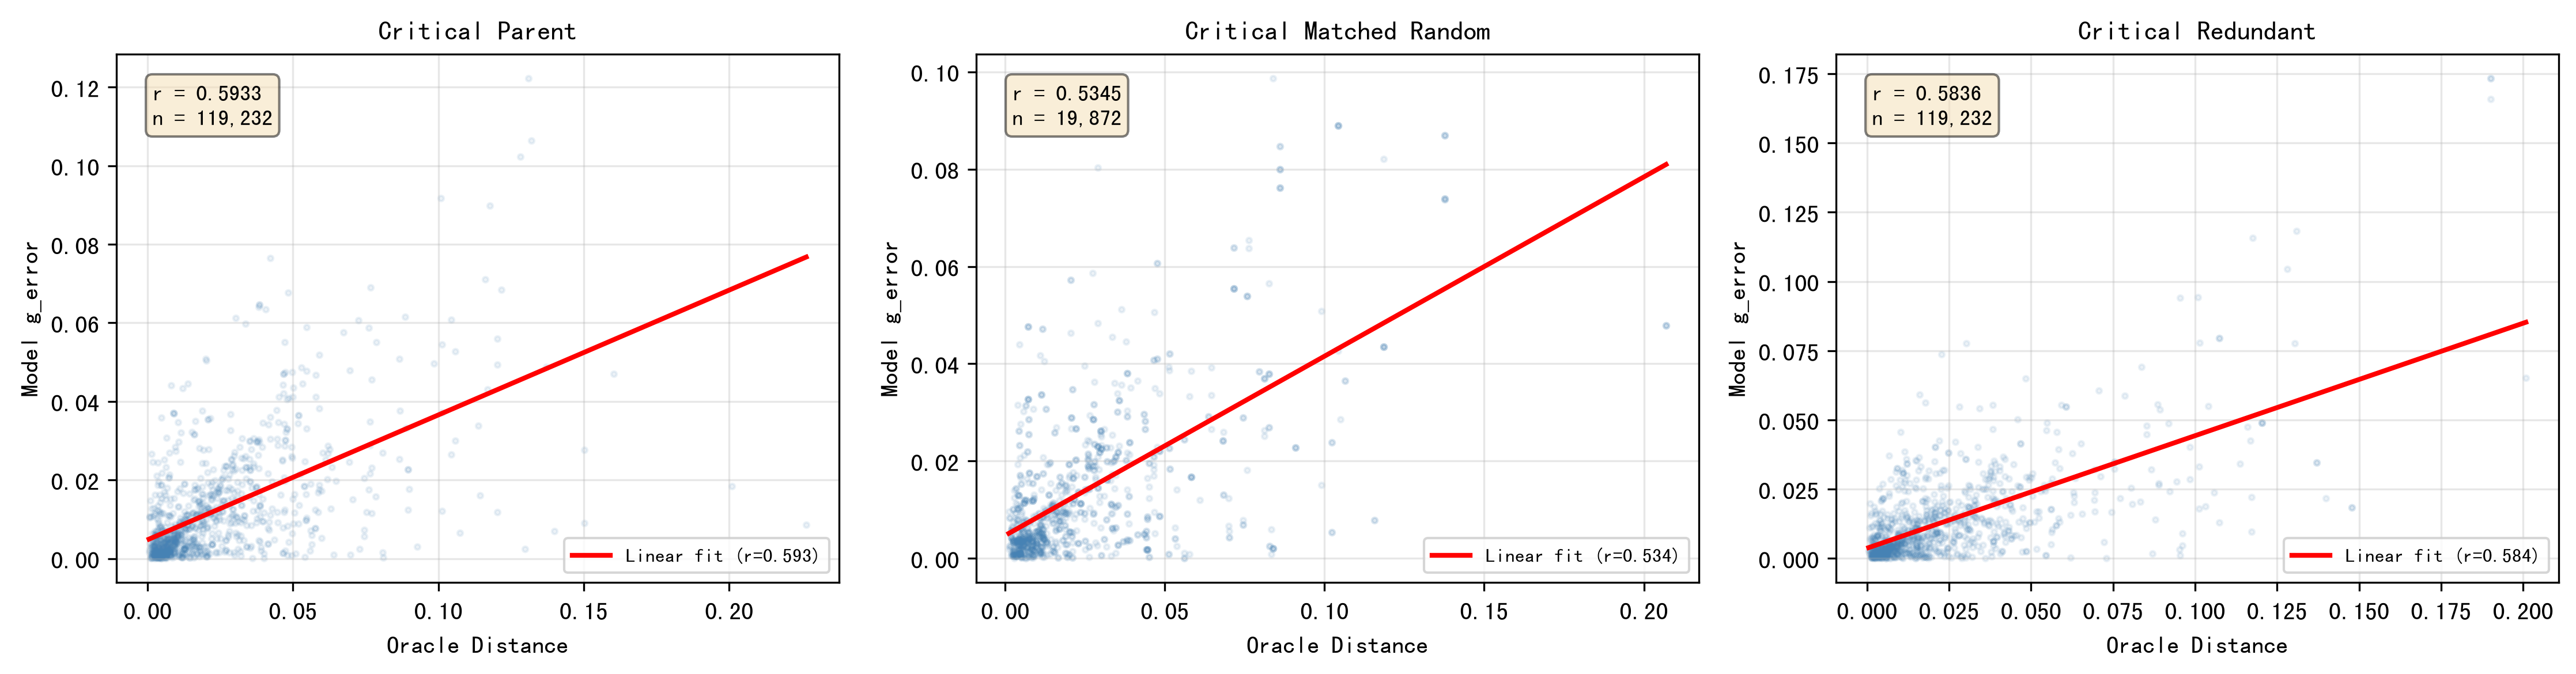
\includegraphics[width=\linewidth]{figures/b1_oracle_correlation_figure.png}
  \caption{\textbf{Oracle-relative geometry error across deletion pair classes.} Each panel shows the association between oracle distance and $E_{\mathrm{geometry}}=|d_{\mathrm{model}}-d_{\mathrm{oracle}}|$ for PROP-DIRECT across 1,000 randomly sampled test cases. Left: Critical vs. full sensor complement ($r=0.5933$). Center: Critical vs. matched random deletion ($r=0.5345$). Right: Critical vs. redundant deletion ($r=0.5836$). The correlations are descriptive because cases share assets and query structure; they do not establish a new confirmatory endpoint.}
  \label{fig:b1-correlation}
\end{figure}

The critical-vs-random association is 9.9\% weaker than the critical-vs-full association. We treat this contrast as an exploratory pattern in oracle-relative error; the paired cases share assets and query structure.

\subsubsection{Baseline Comparison: Architecture-Specific Limitation}

The standard baseline (B-STDPROB) exhibits the opposite pattern:
\begin{itemize}
    \item \textbf{Critical vs. Full:} $r = 0.6606$
    \item \textbf{Critical vs. Random:} $r = 0.6732$
\end{itemize}

For B-STDPROB, the matched-random correlation is stronger. The contrast associates the weaker-correlation pattern with PROP-DIRECT's sensor-set conditioning pathway rather than with prognostic models in general.

\subsubsection{Interpretation}

The residual analysis suggests that PROP-DIRECT approximates the oracle-defined geometry about as closely as the baseline in the critical-versus-full comparison, with a larger point estimate under matched-random deletion. Together with the pair-class ordering, this indicates that the availability signal is easier to represent than the functional distinctions among sensors. The evidence is diagnostic rather than a proof that either model has the correct posterior geometry in every case.

\subsection{Prediction Quality and Calibration}
\label{sec:results:quality}

\subsubsection{Predictive quality and posterior geometry}

We compared standard prognostic quality metrics across all seven model variants in the frozen model suite. Table~\ref{tab:c2_quality} reports asset-level macro-averages on the information-loss evaluation, which is scored under a separate frozen contract covering the full 96-asset population (Section~\ref{sec:methods:protocol}); it is distinct from the 10-asset test/lockbox partition used for the sufficient-observation claims.

\begin{table}[tb]
  \centering
  \caption{Descriptive predictive quality under information loss
  (covering the full 96-asset population; distinct from the 10-asset
  test/lockbox partition described in
  Section~\ref{sec:methods:protocol}). Values are means within asset followed
  by means over 96 assets; lower is better.}
  \label{tab:c2_quality}
  \resizebox{\linewidth}{!}{%
    \begin{tabular}{lrrrrrr}
      \toprule
      Model & State MAE & Failure MAE & CRPS & State rank & Failure rank & CRPS rank \\
      \midrule
      \propdirect{} & 0.014577 & 0.069585 & 0.048445 & 3 & 3 & 2 \\
      \bstdprob{}   & 0.014462 & 0.069195 & 0.048038 & 2 & 1 & 1 \\
      B-INDEP       & 0.014881 & 0.070197 & 0.049115 & 5 & 5 & 5 \\
      B-INVAR       & 0.014847 & 0.069970 & 0.048645 & 4 & 4 & 3 \\
      B-CDE         & 0.015563 & 0.070610 & 0.049103 & 6 & 6 & 4 \\
      B-SET         & 0.017344 & 0.071081 & 0.049566 & 7 & 7 & 7 \\
      B-WIDEN       & 0.014455 & 0.069255 & 0.049189 & 1 & 2 & 6 \\
      \bottomrule
    \end{tabular}%
  }
\end{table}


PROP-DIRECT ranks third for both state mean absolute error (MAE) and failure-time MAE, and second for CRPS among the seven models. Its CRPS difference from B-STDPROB is $+4.07 \times 10^{-4}$.

The quality table separates predictive accuracy from cross-view geometry: PROP-DIRECT remains competitive on single-view metrics even where its geometric advantage disappears. The C-MAPSS analysis next asks whether this distinction is visible on a public simulated benchmark.

\subsubsection{Posterior Calibration}
\label{sec:results:calibration}

We next use the frozen C1 posterior samples for a descriptive calibration check. The central intervals are close to their nominal levels on both held-out splits: the mean 90\% coverage across the three coordinates is 0.909 for PROP-DIRECT on test and 0.902 on lockbox, compared with 0.913 and 0.903 for B-STDPROB. The PIT histograms are likewise close to the uniform reference (Figure~\ref{fig:calibration}); the small differences do not support a claim that either method is uniformly better calibrated. This result separates the paper's primary geometric finding from posterior reliability: the conditioning mechanism improves cross-view geometry under sufficient observation while calibration remains broadly comparable to the baseline.

\begin{table}[tb]
\centering
\caption{\textbf{Posterior calibration diagnostics on the C1 evaluation splits.} Coverage entries are averaged over the three joint coordinates and include 90\% asset-bootstrap intervals. PIT histogram L1 is a descriptive distance from a uniform histogram; zero is ideal.}
\label{tab:calibration}
\begin{tabular}{llcc}
\toprule
Model & Split & 90\% coverage & PIT histogram L1 \\
\midrule
\propdirect{} & test & 0.909 [0.888, 0.928] & 0.082 \\
\propdirect{} & lockbox & 0.902 [0.877, 0.925] & 0.084 \\
\bstdprob{} & test & 0.913 [0.894, 0.931] & 0.084 \\
\bstdprob{} & lockbox & 0.903 [0.877, 0.927] & 0.085 \\
\bottomrule
\end{tabular}
\end{table}


\begin{figure}[!ht]
  \centering
  \includegraphics[width=0.94\linewidth]{fig7_calibration_reliability.png}
  \caption{\textbf{Posterior calibration diagnostics.} Left: empirical central coverage at nominal 50\%, 80\%, and 90\% levels, averaged over the three joint coordinates. Right: PIT histograms with the uniform reference shown by the dashed line. Circles and squares denote test and lockbox splits; the plots are descriptive checks rather than additional decision gates.}
  \label{fig:calibration}
\end{figure}

% Protocol-aligned benchmark evaluation. FD001 is simulated and uses artificial
% sensor deletion; it is reported as benchmark evidence rather than field validation.
\subsection{Conditional Cross-View Geometry on C-MAPSS}
\label{sec:results_cmapss}

To test the geometric hypothesis under the shared-model protocol, we evaluated PROP-DIRECT and B-STDPROB on C-MAPSS FD001~\citep{saxena2008cmapss}. FD001 contains 100 training and 100 test engine trajectories generated by NASA's Commercial Modular Aero-Propulsion System Simulation, with 14 non-constant sensor channels after preprocessing. It provides a public simulated reference for the analysis, while remaining distinct from field data.

\subsubsection{Shared-model protocol}

We retained the full 14-channel view and formed two reduced views by deleting three channels from each (11 channels per view; the two deletion sets differ by six channels). For each method, a single model was trained on the union of all three masked views. The 100 training engines were split by engine into 80 fitting and 20 validation engines, so views of the same engine remained in one split. The models use the MSE point-prediction head implemented for this benchmark; 128 dropout passes at test time provide predictive samples. We evaluate the final window of each of the 100 test engines and report energy distances on the raw RUL scale.

\subsubsection{Agreement depends on the view pair}

Table~\ref{tab:cmapss_validation} shows a conditional pattern. PROP-DIRECT reduces the distance to the full view by 18.5\% (90\% CI: 7.8--29.3\%) for View 1 and by 28.9\% (18.4--37.9\%) for View 2. For the two reduced views, however, the ordering reverses: PROP-DIRECT has a 36.6\% larger distance than B-STDPROB (90\% CI: $-62.9$ to $-13.1$\%). The shared model therefore aligns predictions when a reduced view is compared with the full sensor complement, but it does not maintain that alignment when two equally sized views differ in sensor identity.

% Table: C-MAPSS benchmark evaluation (shared-model regime, quality-controlled)
\begin{table}[t]
\centering
\begin{threeparttable}
\caption{\textbf{Cross-view energy distances on the C-MAPSS FD001 simulated
turbofan benchmark under the shared-model protocol.} A single model per
architecture is trained on data that mixes all three observation
configurations, mirroring the synthetic protocol. Lower energy distance
indicates closer agreement between dropout-sampled predictive distributions
for the same engine viewed under different sensor configurations; distances
are on the raw RUL scale (cycles). Bootstrap 90\% confidence intervals in
brackets (2,000 replicates, resampling engines). Negative relative reduction
indicates PROP-DIRECT is \emph{worse}.}
\label{tab:cmapss_validation}
\begin{tabular}{lccc}
\toprule
\textbf{View Pair} & \textbf{PROP-DIRECT} & \textbf{B-STDPROB} & \textbf{Relative Reduction} \\
\midrule
Full vs.\ View 1    & 1.85 [1.61, 2.11] & 2.27 [2.04, 2.51] & 18.5\% [7.8\%, 29.3\%] \\
Full vs.\ View 2    & 1.80 [1.56, 2.05] & 2.54 [2.29, 2.79] & 28.9\% [18.4\%, 37.9\%] \\
View 1 vs.\ View 2  & 1.85 [1.57, 2.17] & 1.36 [1.19, 1.52] & $-36.6$\% [$-62.9$\%, $-13.1$\%] \\
\bottomrule
\end{tabular}
\begin{tablenotes}
\footnotesize
\item Single-view test MAE (cycles), same runs: PROP-DIRECT 16.44 (full) /
15.95 (View 1) / 16.25 (View 2); B-STDPROB 16.27 (full) / 15.42 (View 1) /
15.73 (View 2). The near-identical point accuracy makes this geometry
comparison quality-controlled: differences in cross-view distance cannot be
attributed to differences in posterior informativeness.
\end{tablenotes}
\end{threeparttable}
\end{table}


The single-view MAEs are close across methods. PROP-DIRECT obtains 16.44, 15.95, and 16.25 cycles for the full, View 1, and View 2 conditions, compared with 16.27, 15.42, and 15.73 for B-STDPROB. The reversal in the reduced-view pair is consequently not explained by a large point-accuracy collapse. It is consistent with a more specific sensitivity to which sensors are present, although the benchmark has no oracle posterior with which to identify the mechanism.

This shared-model result is stronger evidence than the earlier specialist comparison because the conditioning pathway is trained across views, but it remains evidence from a simulated benchmark with artificial deletion. It supports a conditional extension of the synthetic finding and sharpens the importance-awareness boundary; it does not establish performance under naturally occurring sensor loss. The archived protocol and outputs make a future study with domain-informed critical channels and field data possible.

